\item \textbf{{[}ALVL/9597/2016/P2/Q2{]} }

A firm hires vehicles to customers. A customer usually makes a booking
a number of weeks before the start of the hire period. The customer
pays a deposit at the time of the booking and the balance when they
return the vehicle from hire.

At the time of the booking, the firm records the following data:
\begin{itemize}
\item customer data, including a customer reference code
\item booking date
\item hire start date
\item hire return date
\item type of vehicle
\item deposit taken
\end{itemize}
Vehicle types are coded as follows:
\begin{itemize}
\item Small car - SC
\item Large car - LC
\item Utility vehicle - UV
\end{itemize}
Each vehicle type has its own daily charge, for each day of the hire
period.

Each vehicle has a unique registration.

Customers may make more than one booking. The software will not allow
a customer to make more than one booking for the same start date.

The document below is an example of an invoice printed for the customer
when they return the vehicle and pay the balance due.
\begin{center}
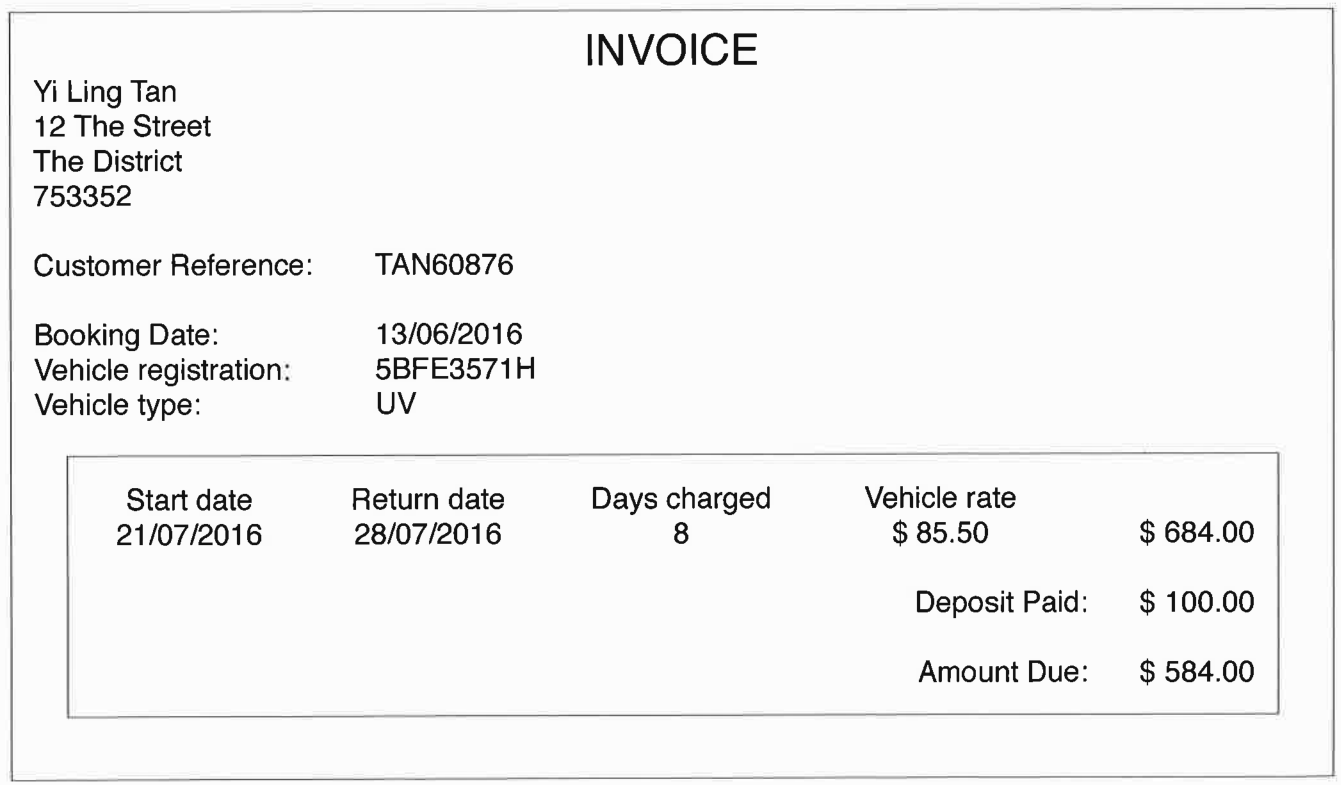
\includegraphics[width=0.5\paperwidth]{C:/Users/Admin/Desktop/Github/question_bank/static/img/9597-ALVL-2016-P2-Q2}
\par\end{center}
\begin{enumerate}
\item The firm wants to model this application using a relational database.
\begin{enumerate}
\item A database needs a number of tables to store the data for this application.
Draw the Entity-Relationship (E-R) diagram showing the tables and
the relationships between them. \hfill{}{[}6{]}
\item A table description can be expressed as: 

\texttt{TableName (}\texttt{\uline{Attributel}}\texttt{ , Attribute2
, Attribute3 , ....) }

The primary key is indicated by underlining one or more attributes. 

Write table descriptions for the tables you identified in \textbf{part
(i)}. \hfill{}{[}6{]}
\end{enumerate}
\item The firm implements the relational database using a Database Management
System (DBMS). It writes programs to access the data using a Graphical
User Interface (GUI). 

One program is for recording a new booking. 

The firm uses different types of components in a GUI for the display
and entry of data. 

Name \textbf{three} types of component that the booking form could
use and give the types of data it is used to capture. \hfill{} {[}3{]}
\end{enumerate}